\def\year{2022}\relax
%File: formatting-instructions-latex-2022.tex
%release 2022.1
\documentclass[letterpaper]{article} % DO NOT CHANGE THIS
\usepackage{amsmath}
\usepackage[table]{xcolor}
\usepackage{makecell}
\usepackage{floatrow}
\floatsetup[table]{capposition=top}
\newfloatcommand{capbtabbox}{table}[][\FBwidth]
\usepackage{aaai22}  % DO NOT CHANGE THIS
\usepackage{times}  % DO NOT CHANGE THIS
\usepackage{helvet}  % DO NOT CHANGE THIS
\usepackage{courier}  % DO NOT CHANGE THIS
\usepackage[hyphens]{url}  % DO NOT CHANGE THIS
\usepackage{graphicx} % DO NOT CHANGE THIS
\urlstyle{rm} % DO NOT CHANGE THIS
\def\UrlFont{\rm}  % DO NOT CHANGE THIS
\usepackage{natbib}  % DO NOT CHANGE THIS AND DO NOT ADD ANY OPTIONS TO IT
\usepackage{caption} % DO NOT CHANGE THIS AND DO NOT ADD ANY OPTIONS TO IT
\DeclareCaptionStyle{ruled}{labelfont=normalfont,labelsep=colon,strut=off} % DO NOT CHANGE THIS
\frenchspacing  % DO NOT CHANGE THIS
\setlength{\pdfpagewidth}{8.5in}  % DO NOT CHANGE THIS
\setlength{\pdfpageheight}{11in}  % DO NOT CHANGE THIS
%
% These are recommended to typeset algorithms but not required. See the subsubsection on algorithms. Remove them if you don't have algorithms in your paper.
\usepackage{algorithm}
\usepackage{algorithmic}

%
% These are are recommended to typeset listings but not required. See the subsubsection on listing. Remove this block if you don't have listings in your paper.
\usepackage{newfloat}
\usepackage{listings}
\lstset{%
	basicstyle={\footnotesize\ttfamily},% footnotesize acceptable for monospace
	numbers=left,numberstyle=\footnotesize,xleftmargin=2em,% show line numbers, remove this entire line if you don't want the numbers.
	aboveskip=0pt,belowskip=0pt,%
	showstringspaces=false,tabsize=2,breaklines=true}
\floatstyle{ruled}
\newfloat{listing}{tb}{lst}{}
\floatname{listing}{Listing}
%
%\nocopyright
%
% PDF Info Is REQUIRED.
% For /Title, write your title in Mixed Case.
% Don't use accents or commands. Retain the parentheses.
% For /Author, add all authors within the parentheses,
% separated by commas. No accents, special characters
% or commands are allowed.
% Keep the /TemplateVersion tag as is
\pdfinfo{
/Title (AAAI Press Formatting Instructions for Authors Using LaTeX -- A Guide)
/Author (AAAI Press Staff, Pater Patel Schneider, Sunil Issar, J. Scott Penberthy, George Ferguson, Hans Guesgen, Francisco Cruz, Marc Pujol-Gonzalez)
/TemplateVersion (2022.1)
}

% DISALLOWED PACKAGES
% \usepackage{authblk} -- This package is specifically forbidden
% \usepackage{balance} -- This package is specifically forbidden
% \usepackage{color (if used in text)
% \usepackage{CJK} -- This package is specifically forbidden
% \usepackage{float} -- This package is specifically forbidden
% \usepackage{flushend} -- This package is specifically forbidden
% \usepackage{fontenc} -- This package is specifically forbidden
% \usepackage{fullpage} -- This package is specifically forbidden
% \usepackage{geometry} -- This package is specifically forbidden
% \usepackage{grffile} -- This package is specifically forbidden
% \usepackage{hyperref} -- This package is specifically forbidden
% \usepackage{navigator} -- This package is specifically forbidden
% (or any other package that embeds links such as navigator or hyperref)
% \indentfirst} -- This package is specifically forbidden
% \layout} -- This package is specifically forbidden
% \multicol} -- This package is specifically forbidden
% \nameref} -- This package is specifically forbidden
% \usepackage{savetrees} -- This package is specifically forbidden
% \usepackage{setspace} -- This package is specifically forbidden
% \usepackage{stfloats} -- This package is specifically forbidden
% \usepackage{tabu} -- This package is specifically forbidden
% \usepackage{titlesec} -- This package is specifically forbidden
% \usepackage{tocbibind} -- This package is specifically forbidden
% \usepackage{ulem} -- This package is specifically forbidden
% \usepackage{wrapfig} -- This package is specifically forbidden
% DISALLOWED COMMANDS
% \nocopyright -- Your paper will not be published if you use this command
% \addtolength -- This command may not be used
% \balance -- This command may not be used
% \baselinestretch -- Your paper will not be published if you use this command
% \clearpage -- No page breaks of any kind may be used for the final version of your paper
% \columnsep -- This command may not be used
% \newpage -- No page breaks of any kind may be used for the final version of your paper
% \pagebreak -- No page breaks of any kind may be used for the final version of your paperr
% \pagestyle -- This command may not be used
% \tiny -- This is not an acceptable font size.
% \vspace{- -- No negative value may be used in proximity of a caption, figure, table, section, subsection, subsubsection, or reference
% \vskip{- -- No negative value may be used to alter spacing above or below a caption, figure, table, section, subsection, subsubsection, or reference

\setcounter{secnumdepth}{0} %May be changed to 1 or 2 if section numbers are desired.

% The file aaai22.sty is the style file for AAAI Press
% proceedings, working notes, and technical reports.
%

% Title

% Your title must be in mixed case, not sentence case.
% That means all verbs (including short verbs like be, is, using,and go),
% nouns, adverbs, adjectives should be capitalized, including both words in hyphenated terms, while
% articles, conjunctions, and prepositions are lower case unless they
% directly follow a colon or long dash
\title{Dual Energy-Flow Enhanced Graph Neural Network\\ for Visual Question Answering}
\author{
    %Authors
    % All authors must be in the same font size and format.
    Written by AAAI Press Staff\textsuperscript{\rm 1}\thanks{With help from the AAAI Publications Committee.}\\
    AAAI Style Contributions by Pater Patel Schneider,
    Sunil Issar,\\
    J. Scott Penberthy,
    George Ferguson,
    Hans Guesgen,
    Francisco Cruz\equalcontrib,
    Marc Pujol-Gonzalez\equalcontrib
}
\affiliations{
    %Afiliations
    \textsuperscript{\rm 1}Association for the Advancement of Artificial Intelligence\\
    % If you have multiple authors and multiple affiliations
    % use superscripts in text and roman font to identify them.
    % For example,

    % Sunil Issar, \textsuperscript{\rm 2}
    % J. Scott Penberthy, \textsuperscript{\rm 3}
    % George Ferguson,\textsuperscript{\rm 4}
    % Hans Guesgen, \textsuperscript{\rm 5}.
    % Note that the comma should be placed BEFORE the superscript for optimum readability

    2275 East Bayshore Road, Suite 160\\
    Palo Alto, California 94303\\
    % email address must be in roman text type, not monospace or sans serif
    publications22@aaai.org
%
% See more examples next
}

%Example, Single Author, ->> remove \iffalse,\fi and place them surrounding AAAI title to use it
\iffalse
\title{My Publication Title --- Single Author}
\author {
    Author Name
}
\affiliations{
    Affiliation\\
    Affiliation Line 2\\
    name@example.com
}
\fi

\iffalse
%Example, Multiple Authors, ->> remove \iffalse,\fi and place them surrounding AAAI title to use it
\title{My Publication Title --- Multiple Authors}
\author {
    % Authors
    First Author Name,\textsuperscript{\rm 1}
    Second Author Name, \textsuperscript{\rm 2}
    Third Author Name \textsuperscript{\rm 1}
}
\affiliations {
    % Affiliations
    \textsuperscript{\rm 1} Affiliation 1\\
    \textsuperscript{\rm 2} Affiliation 2\\
    firstAuthor@affiliation1.com, secondAuthor@affilation2.com, thirdAuthor@affiliation1.com
}
\fi


% REMOVE THIS: bibentry
% This is only needed to show inline citations in the guidelines document. You should not need it and can safely delete it.
\usepackage{bibentry}
% END REMOVE bibentry

\begin{document}

\maketitle

\begin{abstract}
Scene Graphs (SG), the structural abstraction of natural images, contain massive detailed information. The visual reasoning model with SG can significantly improve the ability of reasoning and SG can strengthen the reasoning interpretability. However, existing models often fail to exploit objects, relations, and attributes information jointly in SG, nor can they balance the importance of objects and relations. In this paper, we introduce a novel Dual Energy-Flow Enhanced Graph Neural Network (DE-GNN), which learns a comprehensive representation encoding full-scale scene graph information from objects, attributes, and relations.
Specifically, two types of SG structures are injected into the encoder: (i) \textit{Object-significant graphs} which absorb attribute and relation information into nodes' representations.  (ii) \textit{Relation-significant graphs} which intensify the model's perception of relation features. In addition, we design an \textit{energy-flow mechanism} to enhance the information transfer from edges and adjacent nodes to the updating nodes. We conduct extensive experiments on public GQA and Visual Genome datasets and achieve new state-of-the art performances.
% Evaluated on public GQA and Visual Genome datasets, our method is able to outperform previous state-of-the-art models on these two datasets.
\footnote{our code is available at anonymous github}
% \footnote{\href{https://anonymous.4open.science/r/dual_ggnn-for-vqa-CEDC/}{Our code is available at anonymous github}}
\end{abstract}

\section{Introduction}
Recent developments in deep learning have accelerated the research of Computer Vision (CV) and Natural Language Processing (NLP) areas. Multimodal fusion tasks between image and text have attracted more attention, such as image caption and visual question answering (VQA). The task of VQA requires a model to answer a free-form natural language question using image information. It is a vital multimodal task that has various applications such as AI assistants, multimodal customer service dialogue and image-based search. 

\begin{figure}[ht] 
    \vspace{-0.1in}
    \centering 
    \includegraphics[scale=0.5]{./pic/intro.pdf} 
    \vspace{-0.1in}
    \caption{Visualization of a scene graph with objects, attributes, and relations information} 
    \label{scene-graph} 
    \vspace{-0.2in}
\end{figure}

Scene graph reasoning is an important branch of VQA tasks~\cite{DBLP:journals/corr/abs-2007-01072}. 
To generate the scene graph, the model extracts objects' names, attributes and relationships from the images and constructs them into graph representation as illustrated in Figure~\ref{scene-graph}. 
This representation is better than object features extracted from images by convolutional neural network (CNN) since it is in text form~\cite{DBLP:journals/corr/abs-2101-05479}, and graph architecture has greater interpretability~\cite{DBLP:conf/bmvc/ZhangCX19}.
Two reasoning methods on scene graphs are proposed: (i) Take scene graphs as probabilistic graphs and iteratively update nodes' probabilities using soft instructions extracted from questions such as Neural State Machine (NSM)~\cite{DBLP:conf/nips/HudsonM19,DBLP:conf/ijcnn/LeLV020}; (ii) Apply Graph Neural Network (GNN) into scene graph~\cite{inproceedings,DBLP:conf/iccv/LiGCL19} to learn a joint representation of the nodes and the relations, and then feed the representation into a predictor to get answer.
\begin{figure*}[ht] 
    \vspace{-0.5in}
    \centering 
    \includegraphics[width=1.0\textwidth]{./pic/DE-GNN.pdf} 
    % \vspace{-0.1in}
    \caption{Model structure of the proposed Dual Energy-Flow enhanced Graph Neural Networks. EF is the energy-flow module. Images are transformed into scene graphs by the scene graph generator. The object-significant form and relation-significant form of the scene graph are injected into object encoder and relation encoder. Nodes' representations are generated from the sum of energy-flow modules. The representations will be fused with question representation to predict an answer.} 
    \label{fig2} 
    \vspace{-0.2in}
\end{figure*}
These scene graph reasoning frameworks have been proven useful in VQA tasks. However, none of the existing methods fully utilize the scene graph information, including objects, attributes, and relations, neither can they generate comprehensive representations for objects using features from their neighbors and their attributes. Information from objects and relations connected to them is reconstructed into object features in GNN-based methods. However, these encoding methods miss information from objects' attributes and objects on the other side of edges. The NSM methods use attention mechanisms to update answer possibilities of objects, attributes, and relations, but they cannot learn the joint representation of all three information. What's more, GNN-based models and NSM models are more focused on object features, and taking relation features as references. Empirically, we demonstrate that a correct relation representation is crucial to the VQA task. All these inefficient usages of scene graph information lead to the bottleneck of VQA.

Motivated by this, we propose the Dual Energy-Flow Enhanced Graph Neural Network (DE-GNN) for VQA, introducing a novel scene graph reasoning model that extracts full-scale feature maps from objects, attributes, and relations information in scene graphs. Concretely, as shown in Figure~\ref{fig2}, our DE-GNN model contains a scene graph generator, a question encoder, dual graph encoders, and a fusion module. Firstly, the scene graph generator extracts graphs out of images. Secondly, to preserve integrated information in the encoding process, we transform scene graphs into a relation-significant modality, in which nodes represent relations and edges represent objects, and an object-significant modality, in which nodes represent objects and edges represent relations. Lastly, after receiving scene graphs in two modalities, dual graph encoders can produce feature maps focusing on both relations and objects.

Furthermore, to learn a node's joint representation from its attributes, edges, and adjacent nodes, we modify the gated graph neural network (GGNN) structure in DE-GNN by adding the energy-flow module. It is a  bidirectional GRU to guide the internal information flow.
The encoder can capture information from nodes, edges, and adjacent nodes that connect to them. The outputs of encoder pass through multi-head attention layers with question features from the question encoder. In this way, the model can dynamically focus on the critical parts of questions and use the most similar part of the scene graph as the answer.

In summary, our main contributions are as follow:%\vspace{-0.05in}
\begin{itemize}
\setlength{\itemsep}{5pt}
\setlength{\parsep}{5pt}
\setlength{\parskip}{5pt}
\item We propose a novel DE-GNN model to learn a comprehensive representation of scene graphs by encoding graphs' object-significant modality and relation-significant modality.\vspace{-0.06in}

\item Our energy-flow module is more suitable for processing graphs with meaningful edges and nodes with internal attributes.\vspace{-0.06in}

\item We conduct experiments on GQA and Visual Genome and experimental results demonstrate the effectiveness of DE-GNN which can improve the reasoning accuracy on semantically complicated questions.
% \item We show that our method outperforms other SG-based models in four scene graph datasets, which are generated from the VG dataset by four scene graph generation methods. Extensive experiments demonstrate the effectiveness of DE-GNN.
\end{itemize}\vspace{-0.06in}

\section{Related Works}
\noindent\textbf{Visual Question Answering.}
Most VQA approaches utilize a question encoder architecture that can learn complex temporal dynamics using a sequence of hidden states. To encode the image, most VQA approaches employ CNN-based pretrained models like Mask-RCNN or Faster-RCNN~\cite{DBLP:conf/cvpr/FanZ18,DBLP:conf/cvpr/PatroN18,DBLP:conf/cvpr/NamHK17}. The image encoder and question encoder then pass through a multimodal fusion part and the output fusion vector pass through an answer predictor.

To learn image representations that more focused on questions, many attention-based models are proposed such as BUTD~\cite{DBLP:conf/cvpr/00010BT0GZ18}, SAT~\cite{DBLP:conf/cvpr/YangHGDS16}, question-guided spatial attention~\cite{DBLP:conf/eccv/XuS16}. In~\citet{DBLP:conf/nips/LuYBP16}, the authors proposed a hierarchical co-attention model that jointly implements both image-guided question attention and question-guided visual attention.  MacNet~\cite{DBLP:conf/iclr/HudsonM18}uses Mac-cells to combine attention and encoding function. However, there still exists a significant semantic gap between image and natural language. Transformer-based models such as Unicoder-VL~\cite{DBLP:conf/aaai/LiDFGJ20} can achieve outstanding performance on VQA tasks, but these models need complicated pretrain strategies and extra datasets. The pretraining tasks are time-consuming and hard to update under the changeable environment. To solve the existing problems in attention-based and transformer-based VQA models, we apply scene graphs as our reasoning model base.

\vspace{0.05in}
\noindent\textbf{Scene Graph Generation and Reasoning.}
Most SGG methods use object detection methods like mask-rcnn or faster-rcnn to extract region proposals from images~\cite{DBLP:conf/cvpr/XuZCF17,DBLP:conf/eccv/YangLLBP18,DBLP:conf/cvpr/ZellersYTC18,DBLP:conf/nips/WooKCK18,DBLP:conf/cvpr/DaiZL17,DBLP:conf/iccv/LiOZWW17,DBLP:conf/eccv/YinSLYWSL18}. Methods to reduce the SGG training bias has been put forward~\cite{DBLP:conf/cvpr/TangNHSZ20}. Due to the graph hierarchy extracted from images, SG can promotes explainable reasoning for downstream multimodal tasks such as VQA~\cite{DBLP:conf/bmvc/ZhangCX19}. In our work, scene graph generation methods are used to transform VQA datasets into scene graph datasets. Our model is then tested in datasets generated by different SGG methods.

In typical scene graph reasoning models, neural state machine~\cite{DBLP:conf/nips/HudsonM19} first predict a scene graph that represents its underlying semantics and serves as a structured world model. Then it performs sequential reasoning over the graph, iteratively traversing its nodes to answer a given question or draw a new inference. But state machine-based models can't effectively capture complicated scene graph features. FSTT~\cite{inproceedings} uses GGNN based model to encode scene graphs but it neglects vital information from edges and attributes. Relation-aware Graph Attention Network~\cite{DBLP:conf/iccv/LiGCL19} encodes each image into a graph and models multitype inter-object relations via a graph attention mechanism, to learn question-adaptive relation representations. However, neither can it fully use attribute information nor can it learn the comprehensive representation of scene graphs using graph attention network. Our model uses GGNN structure to learn more comprehensive scene graph representations. 

\vspace{0.05in}
\noindent\textbf{Graph Neural Network.}
GNN~\cite{DBLP:journals/tnn/ScarselliGTHM09} extended traditional neural networks into graph domains. A group of graph-based models~\cite{DBLP:conf/aaai/0001RFHLRG19,DBLP:conf/aaai/LiuCLZLSQ19} were proposed for different graph tasks including graph representation learning. Inspired by convolution neural network, GCN~\cite{DBLP:conf/iclr/KipfW17} improves efficiency with fast approximated spectral operations. GAT~\cite{DBLP:conf/iclr/VelickovicCCRLB18} introduced the attention mechanism to GNN, leveraging masked self-attentional layers to address the shortcomings of prior methods based on graph convolutions or their approximations. GGNN~\cite{DBLP:journals/corr/LiTBZ15} uses gated recurrent units to accelerate the training speed and gain favorable inductive biases on large-scaled graphs.
\cite{DBLP:conf/cncl/WangGCL16,DBLP:conf/aaai/WangCGL18,DBLP:conf/aistats/SunL19} apply GNN-based models on knowledge graphs, which similar to scene graphs.
However, existing GNN-based models cannot effectively process graphs with node attributes and complicated labels. Our DE-GNN model can learn a comprehensive representation using full-scale scene graph information from objects, attributes, and relations to overcome these problems.

\section{Methodolegy}

First we define the VQA task: a classification model learning to answer questions about a given image. Given questions \emph{q} and images \emph{m}, the model maximize a conditional distribution over candidate answers \emph{a}:
\begin{equation}
    \hat{a} = \mathop{\arg\max}_{a \in A}p_\theta(a|q, m)
\end{equation}
where \emph{A} is the set of all possible answers, $p_\theta$ represents the VQA model with the trainable parameter $\theta$ and $\hat{a}$ is the final answer.

Our proposed architecture to solve the VQA task is shown in Figure~\ref{fig2}. Our model contains a scene graph generator, a question encoder, dual graph encoders and a fusion module. For the scene graph generator, we follow the method by \cite{tang2020sggcode} and other three baselines referred in this work, which we will describe in detail later in the experiment section. 
For the question encoder, sementic questions are first embedded by GLOVE pretrained word embedding dataset~\cite{pennington-etal-2014-glove}. After adding a position encoding matrix into questions, we use LSTM to generate questions embedding $q \in R^{dim}$. We'll introduce our dual GGNN encoders in the following subsection.

\subsection{Object/Relation-Significant Graph}
We organize scene graphs into object-significant modality and relation-significant modality. 

\textbf{Object-Significant Graph.} We define the object-significant modality as $\emph{G}_{obj}$, every nodes represent objects in the image and every edges represent relations between two objects. Define $\emph{N}$ as the node set and $\emph{E}$ as the edge set. For $n_i, n_j \in \emph{N}$, $e_k \in \emph{E}$, < $n_i$ - $e_k$ - $n_j$ > denotes the relation tuple that represents the relation $e_k$ from object $n_i$ to object $n_j$. Noted that relation tuples are not symmetrical: if $<n_i - e_k - n_j>$ is a valid relation tuple,  $<n_j - e_k - n_i>$ may not exist. Also, $n_i$ and $n_j$ may have several relations. 

\textbf{Relation-Significant Graph.} We define relation-significant modality as $\emph{G}_{rel}$, every nodes represent relations appear between objects in the image and every edges represent objects, which is completely opposed to the object-significant modality. For $e_i, e_j \in \emph{E}$, $n_k \in \emph{N}$, $<e_i - n_k - e_j>$ denotes the relation tuple that represents the relation $e_i$ and $e_j$ have a shared object $n_k$. Noted that relation tuples are also not symmetrical.

\textbf{Attribute types.} Define \emph{L} as attribute types (such as material, color, etc). For each node $n_i\in\emph{N}$ that corresponds to an object in the
image, we define a set of $\emph{L}+1$ property variables ${\left\{ n_i^j\right\}}_{l=0}^L$, where $n_i$ represents the object's name embedding and $n^l$ represents the embedding of node's $l^{th}$ attribute.

\subsection{Dual Encoders}

Every input scene graph is transformed into an information tuple ($\emph{N}, \emph{E}, \emph{A}_{in}, \emph{A}_{out}$):
\begin{itemize}
    \item \emph{N} is a collection of node embedding.
    \item \emph{E} is a collection of directed edges that specify valid relation between nodes
    \item $\emph{A}_{in}$ is the adjacency matrix of incident edges
    \item $\emph{A}_{out}$ is the adjacency matrix of output edges
\end{itemize}
Suppose $h_i^t$ is the hidden state of $n_i$ in GGNN timestep $\emph{t}$. When $\emph{t}=0$, we initialize $h_i^0$ as the GLOVE embedding of $n_i$ with appropriate 0 padding:
\begin{equation}
    h_i^0 = [n_i^T, 0]^T 
\end{equation}
The incident edges and output edges are retrieved in adjacency matrix $\emph{A}_{in}$ and $\emph{A}_{out}$. 

\subsubsection{Energy-Flow Module}
To enhance the information transfer from edges and adjacent nodes to the updating nodes, we use the Energy-Flow module (EF) to replace the fully-connected layers from original GGNN model. In the energy-flow module, take $<{n}_i, {e}_k, {n}_j>$as an example, the edge ${e}_k$'s embedding state $e_k$ and neighbor node  ${n}_j$'s hidden state $h_j$ are injected into a bidirectional GRU network as input sequence while the node ${n}_i$'s hidden state $h_i$ is injected as GRU's initial hidden state. The output of GRU represents the updating information for hidden state $h_i$, which is the key information from ${e}_k$ and ${n}_j$ that related to ${n}_i$. The sum of every GRU output is ${n}_i$'s total information gain from ${n}_i$ adjacent nodes and edges. The detailed formula is as follows:
\begin{gather}
    EF_i(A_{in}) = \sum\limits_{k,j}^{<\mathcal{n}_i,\mathcal{e}_k,\mathcal{n}_j>\in A_{in}} \text{GRU}([e_k, h_j], h_i) \\
    EF_i(A_{out}) = \sum\limits_{k,j}^{<\mathcal{n}_j,\mathcal{e}_k,\mathcal{n}_i>\in A_{out}} \text{GRU}([e_k, h_j], h_i)
\end{gather}
where $EF_i(A_{in})$ is ${n}_i$'s incident information gain, and  $EF_i(A_{out})$ is ${n}_i$'s output information gain.

\subsubsection{Propagation Model}

In timestep $t$, the hidden states of all nodes are updated by the following gated propagator module:
\begin{gather}
    k_{i}^t = [EF_i^t(A_{in}), EF_i^t(A_{out})]
\end{gather}
where $k_{i}^t$ represents the node ${n}_i$'s representation from all its incident edges, output edges and adjacent nodes.

% The remaining are 
Then we adopt GRU-like updates to incorporate information from adjacent nodes and from the previous timestep to update each node’s hidden state:
\begin{gather}
    % c_i^t = W_i^T[h_i^{(t-1) T}, k_{i}^{(t-1) T}]^T + b\\
    c_i^t = [h_i^{(t-1)}, k_{i}^{(t-1)}] W + b\\
    z_i^t = \sigma(U^z c_i^t) \\
    r_i^t = \sigma(U^r c_i^t)
\end{gather}
where $W, U^z$ and $U^r$ are refer to as trainable weight matrices and $b$ as bias term, $z_i^t$ and $r_i^t$ are the update and reset gates at timestep $t$.
\begin{gather}
    \tilde{h}_i^t = \text{tanh}(U_1 k_{i}^{(t-1)} + U_2(r_u^t \odot h_i^{(t-1)}))\\
    h_i^t = (1-z_i^t)\odot h_i^{(t-1)} + z_i^t\odot \tilde{h}_i^t
\end{gather}
Here, $U_1$ and $U_2$ are the trainable parameters of the linear layers. The operator $\odot$ denotes element-wise multiplication. $h_i^t$ is the updated hidden state for node ${n}_i$. After \emph{T}  steps, the GGNN encoder generates the final hidden state map $G$ of the graph. Finally, we compute the graph embedding $g_i \in G$ for node ${n}_i$ as follows:
\begin{equation}
    g_i = \sigma( \emph{f}(h_i^T, n_i))
\end{equation}
Here, $\emph{f}$ is the multi-layer perceptron (MLP) layer which receives the concatenation of $h_i^T$ and $n_i$, then generates the final representation of ${n}_i$. 

\subsection{Fusion and Answer Predictor}
After receiving node and relation features from dual encoders, we first fuse attributes into feature maps. For node feature map $G^N$ and relation feature map $G^E$, the fusion feature map $F^N$ and $F^E$ are as
$$ F_i^N =\left\{
    \begin{aligned}
    &[g_i^N, n_i^0]\\
    &....\\
    &[g_i^N, n_i^L]
    \end{aligned}
\right.
$$
\begin{gather}
    F_j^E = [g_j^E, e_j], \hspace{0.2in}
    F = [F^N, F^E]
\end{gather}
where $F_i^N$ is node $i$'s fusion feature. $g_i^N$ is node $i$'s representation from the GGNN encoder. $n_i^0$ to $n_i^L$ are node $i$'s attributes embeddings. $F_j^E$ is edge $j$'s fusion feature. $g_j^E$ is edge $j$'s representation from the GGNN encoder. $e_j$ is edge $j$'s original embedding. The full-scale feature map $F$ is the concatenation of $F^N$ and $F^E$.

After that, the question embedding $\emph{q}$ generated from LSTM encoder and full-scale feature map $F$ are injected into multi-head attention layer, where query is $F$ and $\emph{q}$ is key and values. Scores for every features are calculated. After weighted sum of feature map using the score, we get the reasoning vector $\emph{r}$ from the graph and question.

For the answer prediction module, we adopt the two-layer MLP noted by $f(*)$ as a classifier for the candidate answer set. The input of MLP is the concatenation of $\emph{q}$ and $\emph{r}_i$. This classifier is also applied in many VQA models such as NSM~\cite{DBLP:conf/nips/HudsonM19} and MacNet~\cite{DBLP:conf/nips/LuYBP16}.
\begin{gather}
    r = \text{Attention}(F, q)\\
    % p = \text{softmax}(f(r, q))\\
    \hat{a} = \mathop{\arg\max}(\text{softmax}(f(r, q)))
\end{gather}
% Where $f$ is the MLP layers.

\begin{table*}[htbp]
    \begin{floatrow}
    \capbtabbox{
     \begin{tabular}{ll}
      \hline
      \textbf{Models}&\textbf{Acc.}\\
      \textbf{NSM} & 35.5\% \\ 
      \textbf{FSTT}& 31.6\% \\
      \textbf{Re-GAT}& 54.5\% \\
      \textbf{DE-GNN(Ours)} & \textbf{54.9\%}\\
      \hline
    \end{tabular}
    }{
     \caption{Model accuracy on Motif dataset without question fusion module.}
     \label{model-without-fusion}
    }
    \capbtabbox{
     \rowcolors{1}{blue!10}{white}
     \begin{tabular}{llllll}
       \hline
       \textbf{Models}&\textbf{Binary}&\textbf{Open}&\textbf{Validity}&\textbf{Distribution}&\textbf{Accuracy}\\
    \hline
     Human &91.20 &87.40 &98.90 &- &89.30\\
     BottomUp &66.64 &34.83 &96.18 &5.98 &49.74\\
     MAC &71.23 &38.91 &96.16 &5.34 &54.06\\
     SK T-Brain &77.42 &43.10 &96.26 &7.54 &59.19\\
     PVR &77.69 &43.01 &96.45 &5.80 &59.27\\
     GRN &77.53 &43.35 &96.18 &6.06 &59.37\\
     Dream &77.84 &43.72 &96.38 &8.40 &59.72\\
     LXRT &77.76 &44.97 &96.30 &8.31 &60.34\\
     NSM &78.94 &49.25 &\textbf{96.41} &3.71 &63.17\\
     ReGAT &\textbf{83.57} &62.58 &92.70 &- &70.50\\
     DEGNN(ours) &69.79 &\textbf{72.21} &93.80 &- &\textbf{71.21}\\
    \hline
    \hiderowcolors
    \end{tabular}
    }{
     \caption{Performance on GQA dataset.}
     \label{GQA}
    }
    \end{floatrow}
\end{table*}

\begin{table*}
\centering
    \begin{tabular}{lllll}
    \hline
    \textbf{Models}&\textbf{Baseline} & \textbf{Object-EF}&\textbf{Relation-EF}&\textbf{DE-GNN (Ours)}\\
    \hline
     Acc. & 35.4\% & 39.3\% ($\uparrow$3.9\%) & 38.8\% ($\uparrow$3.4\%) & \textbf{75.2\% ($\uparrow$39.8\%)}  \\
    \hline
    \end{tabular}
\caption{\label{ablation-accuracy}
 Model accuracy on Motif validation dataset for ablation study. The baseline is GGNN original version. EF is our energy-flow enhanced GGNN version. Baseline is DE-GNN's object encoder part without energy-flow module. Object-EF is DE-GNN's object encoder part with energy-flow module. Relation-EF is DE-GNN's relation encoder part with energy-flow module.
}
\end{table*}

\section{Experiment}
\subsection{Datasets}

\textbf{Visual Genome} dataset contains 108,077 images with comprehensively annotated objects, attributes, and relations. Due to the lack of scene graph annotations, we use a SGG codebase~\cite{tang2020sggcode} to generate scene graphs for Visual Genome. In order to comprehensively evaluate our scene graph reasoning method, we use four different SGG methods including Motif~\cite{DBLP:conf/cvpr/ZellersYTC18}, IMP~\cite{DBLP:conf/cvpr/XuZCF17},  vctree~\cite{DBLP:conf/cvpr/TangZWLL19} and unbiased-causal-TDE~\cite{DBLP:conf/cvpr/TangNHSZ20} to generate scene graphs with different qualities and biases. We split the dataset into train, valid, and test sets at $7:1:2$ ratio.

\textbf{GQA} dataset centers around real-world reasoning, scene understanding and compositional question answering. It consists of 113K images and 22M questions of assorted types and varying compositionality degrees, measuring performance on an array of reasoning skills such as object and attribute recognition, transitive relation tracking, spatial reasoning, logical inference and comparisons.

\subsection{Implementation Details}

We use 50-dimensional GLOVE word embeddings dataset~\cite{pennington-etal-2014-glove} to embed words in the scene graph and questions. In order to record the questions' position information, we set up the position encoding matrix $\emph{PE}$:
\begin{gather}
    PE_{\emph{pos}=2\emph{i}} = \sin(\emph{pos}/10000^{2i/d_{model}})\\
    PE_{\emph{pos}=2\emph{i}+1} = \cos(\emph{pos}/10000^{2i/d_{model}})
\end{gather}
where $\emph{pos}$ is the word's position in the question sequence. If $\emph{pos}$ is odd, position information is generated by $\sin$. If not, it's generated by $\cos$. We set $d_{model}$ to be 50.

After adding position information, the question embeddings are injected into a single-directional GRU network. The hidden dimension of GRU is 100, and the dropout rate is 0.2.

In our energy-flow enhanced GGNN encoder, the propagator time step is 5, and we use a bidirectional GRU as our energy-flow module. The hidden dimension of GRU is set to 50, and layer num is 1. 

In the fusion module, we employ a multi-head attention layer with 5 heads and no dropouts. As for the answer predictor, we select top-2000 answer candidates and use 2 MLP layers to be the classifier.

We use Adam as the optimizer of our model, and Cross Entropy Loss as the loss function of our model. Our batch size is 512. The learning rate is dynamic according to the epoch number. We initialize the learning rate to be $1e^{-3}$, and when 30\% epochs finish, the learning rate drops to $2e^{-4}$. When 60\%
epochs finish, the learning rate drops to $4e^{-5}$ and it becomes $8e^{-6}$ after 80\% epochs finish. We train our model and other baselines on a single V100 GPU.

% \begin{figure}[h] 
% \mbox{ \hspace{-0.12in}
%     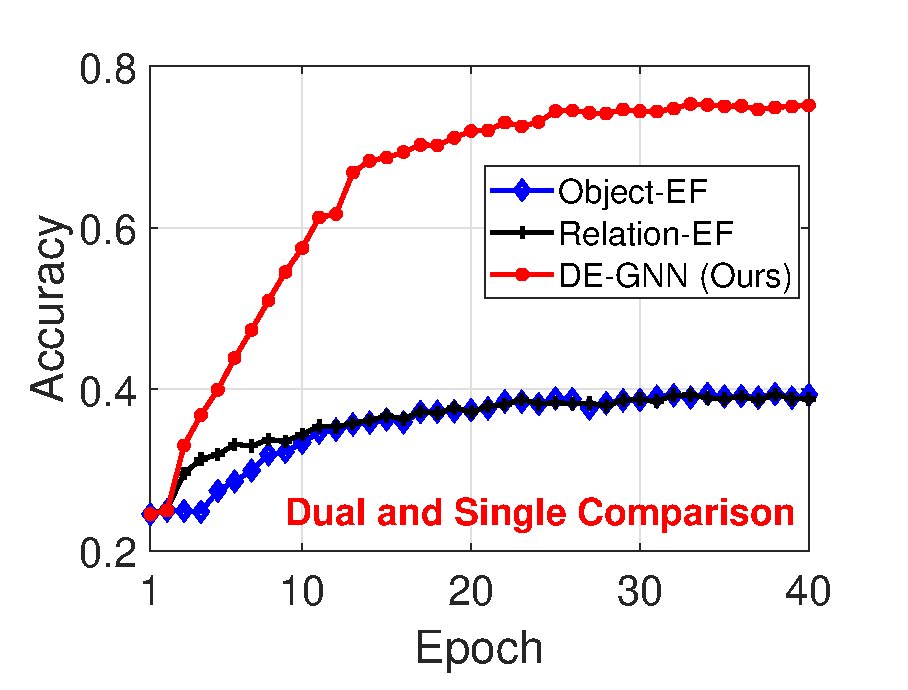
\includegraphics[width=1.6in]{fig/fig5-left.eps} \hspace{-0.12in}
%     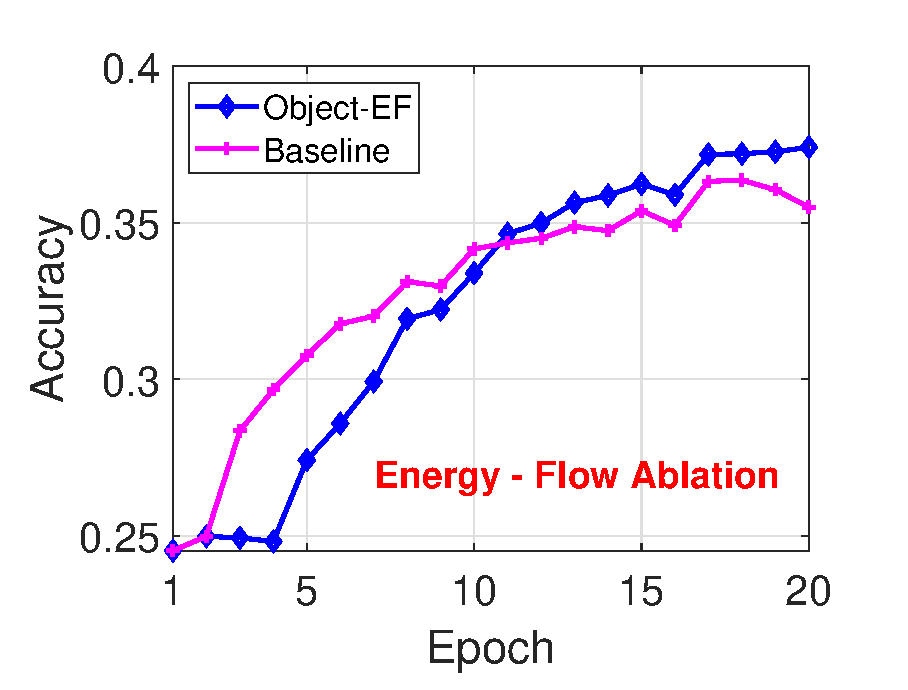
\includegraphics[width=1.6in]{fig/fig5-right.eps} 
% }
%     \caption{The validation accuracy curves for ablation experiments} 
%     \label{ablation-figure} 
% \end{figure}

\begin{table*}
\centering
    \begin{tabular}{l|lllllllll}
    \hline
    \textbf{Question type}&\textbf{What}&\textbf{Color}&\textbf{Where}&\textbf{How}&\textbf{Who}&\textbf{When}&\textbf{Why}&\textbf{Overall}\\
    \hline
     Percentage &(40.9\%) &(19.2\%) &(18.4\%) &(12.0\%) &(3.7\%) &(3.5\%) &(2.0\%) &(100\%)\\
    \hline
      & & & &\makecell[c]{\textbf{VG-GT}}& & & &\\
    \hline
     NSM &0 &0 &0 &0 &0 &0 &0 &45.1\\
     MLP &- &- &- &- &- &- &- &58.5\\
     F-GN &60.9 &53.6 &62.0 &46.2 &63.3 &83.7 &50.9 &60.1\\
     U-GN &61.6 &54.0 &62.4 &45.9 &63.9 &83.2 &50.3 &60.5\\
     SAN &- &- &- &- &- &- &- &62.6\\
     FSTT &38.9 &43.8 &26.8 &28.5 &31.0 &39.0 &16.4 &67.3\\
     ReGAT &45.7 &67.7 &20.5 &49.1 &34.1 &20.4 &20.8 &71.2\\
     DEGNN(ours) &48.5 &63.3 &29.3 &47.4 &43.6 &42.0 &23.1 &76.2\\
    \hline
     & & & &\makecell[c]{\textbf{Motif}}& & & &\\
    \hline
     NSM &0 &0 &0 &0 &0 &0 &0 &43.1\\
     FSTT &31.8 &40.4 &5.7 &34.8 &18.5 &50.3 &3.2 &48.1\\
     ReGAT &56.3 &65.8 &15.1 &62.4 &46.5 &52.3 &24.6 &54.5\\
     F-GN &58.7 &60.8 &60.4 &47.2 &61.8 &84.8 &49.0 &60.0\\
     U-GN &59.4 &58.2 &60.3 &54.3 &66.6 &85.3 &48.1 &60.5\\
     DEGNN(ours) &60.9 &66.2 &20.7 &59.7 &49.0 &58.1 &28.9 &\textbf{72.9}\\
    \hline
    \end{tabular}
\caption{\label{new-detail}
Performance on new dataset in details.
}
\end{table*}

\subsection{Experimental Results}
In this sub-section, we provide experimental results on four scene graph generated datasets mention before. The baselines we compare  use various methods to generate scene graphs for images. To ensure fairness, we reimplement them, removing their scene graph generation parts to eliminate the interference of different generation methods.

Table~\ref{citation-guide} reports results on the test sets of four different datasets generated from the VG dataset. Compared to the baseline models, we can observe that our DE-GNN model outperforms the other baselines. In Motif, Unbias-Causal, and IMP datasets, our model has a 10\% to 20\% improvement in performance.

In addition, the stability of our model is conspicuous. Our model can achieve consistent and stable performance under different scene graph qualities. Our model's performances under four different scene graph datasets only suffer 3\% fluctuation,
while FSTT suffers 4.7\% fluctuation and Re-GAT suffers 26.9\% fluctuation. Figure~\ref{four-graph} is the intuitive validation curves on four datasets. Our model in the blue line can steadily converge at nearly 15 epochs under four different datasets with various scene graph qualities. 

Table~\ref{GQA} reports results on the test sets of the GQA dataset

To demonstrate that our dual encoders structure can intensify the model’s perception of relation features and learn a comprehensive representation from nodes, attributes, and relations information, we make badcase analysis for baselines and our model on Motif dataset. To classify the badcase answer category, we generate three dictionaries to record objects, attributes and relations that appear in scene graphs. For each answer, we first extract potential relations and match them up with the relation dictionary. Then we split the objects and attributes in the answer and search objects and attributes dictionaries. As for some evasive answers containing both objects and its' attributes, we add them in both object and attribute categories. 

Figure~\ref{badcase} shows results on our badcase analysis. Our model surpasses all baselines in the object aspect. Also, our model reduces nearly half of the wrong answers in FSTT, Re-GAT, and NSM in the attribute aspect. Our model also performs well in relation aspect, outperforming GNN based FSTT and Re-GAT.

The question fusion module, which concats the question vector with the reasoning vector before entering into the answer predictor module, commonly appears in VQA models, including NSM, FSTT, and our DE-GNN model. This method can indeed improve the accuracy of VQA models. However, from the cognitive aspect, the question fusion module lacks interpretability because the reasoning vector in the model has included question features. Also, the addition of the question fusion module may lead the reasoning model to "guess answers" from questions, which negatively influences reasoning itself. We retrain our model and other baselines without the question fusion module to evaluate the reasoning ability without the influence of outer question information. Table~\ref{model-without-fusion} shows the results of models without question fusion module. Noted that there is no question fusion module in Re-GAT baseline, so the Re-GAT result is the same as Table~\ref{citation-guide}.
After reducing the concatenation of the question vector and reasoning vector, FSTT, NSM, and our DE-GNN model suffer accuracy recessions. Without question fusion, our model still outperforms other baselines.

\subsection{Ablation Study}

We compare three ablated forms of DE-GNN with our complete one. The accuracy results reported in Table~\ref{ablation-accuracy} are trained using the Motif dataset. The Object-EF model is the object encoder part of our DE-GNN model, which contains one energy-flow enhanced GGNN network to encode object-significant graphs. Oppositely, the relation-EF model is the other half of our DE-GNN model, which contains one energy-flow enhanced GGNN network to encode relation-significant graphs. The baseline model is the original GGNN network to encode object-significant graphs.

Firstly, we validate the effectiveness of applying dual structure to balance the importance of relations and objects by splitting our DE-GNN into the object-single model and the relation-single model. Table~\ref{ablation-accuracy} shows that both object-EF model and relation-EF model perform poorly at about 39\%. It also shows that both relations and objects are vital to VQA performance. Lack of any of them will lead to severe accuracy recession. After combining the object-single model and the relation-single model, we see a gain of approximately 35\% accuracy upward, which shows that the dual structure is significant in balancing relation and object information. 

Secondly, we validate the effectiveness of applying energy-flow structure to learn a more comprehensive representation for scene graphs than the original GGNN structure, which is the baseline in Table~\ref{ablation-accuracy}. We compare the object-EF model and baseline model, which both learn representations from object-significant graphs, and see that after adding the energy-flow structure, there is an accuracy rise at around 3\%. This shows that energy-flow structure can effectively improve the representation quality of scene graphs. 

% To better understand how our dual energy-flow enhanced GNN model inferences and answers questions, we further visualize and compare the attention maps learned by the ablated models in the following subsection.

\subsection{Visualization}
To better illustrate the effectiveness of the dual encoder structure and the energy-flow module in our DE-GNN model, we compare the attention scores learned by DE-GNN model with those learned by our baseline, object-EF, and relation-EF models. Figure~\ref{visual} is the detail of the visualization result. Row 1 is three typical images with questions. 

Comparing the first graph in row 2 with row 3 shows that energy-flow enhanced GGNN encoder can more correctly focus on crucial objects than the original GGNN encoder. For the objects mentioned in the questions, the attention scores of "bus" increase by 0.29. As for objects unrelated to questions, the attention scores of "car" and "tree" decrease by 0.12 and 0.08. The original GGNN encoder can not fuse object and attribute information, which leads to the wrong answer. Our object-EF model learns a jointly representation from objects and attributes. The top-3 candidate attributes for the question are "red", "steel", and "driving". Our object-EF model correctly answers "red".

Comparing the first and third graphs in row 3 with row 4 shows that both object-EF and relation-EF can capture related information, but these models have a significant bias on objects and relations. Relation-EF shows the acute perception on relations, but the model can not capture object information or score objects correctly, which leads to relation-EF's failure on the first graph. The object-EF model can not capture "on" relation in graph 3, while relation-EF model can easily capture the correct answer.

\begin{figure}[h] 
    \flushleft
    \vspace{-0.1in}
    \centering 
    \includegraphics[scale=0.32]{./pic/visual2.pdf} 
    \caption{Visualization of attention scores learned by baseline, object-EF, relation-EF, and DE-GNN.} 
    \label{visual} 
    \vspace{-0.2in}
\end{figure}

Our DE-GNN, which in row 5, can not only balance the importance of objects and relations, but also learn jointly representations from objects, attributes, and relations using the energy-flow module. Comparing the second graph in row 3 and row 5, our model correctly capture "horse" object and "behind" relation. This leads to the correct attention score of "old man", which is 0.61 higher than the score from object-EF. Our model answers three questions correctly.
\section{Conclusion}
In this work, we studied classic scene graph reasoning methods such as GNN-based models and Neural State Machine for VQA. We observed that existing methods fail to exploit nodes, relations, and attributes information jointly in scene graphs. To address this problem, we propose the Dual Energy-Flow Enhanced Graph Neural Network (DE-GNN), which encodes each scene graph into feature representations via object encoder and relation encoder to generate full-scale feature maps using nodes, attributes, and relations information. Our method have shown significant improvement on the VG dataset and achieve new state-of-the-art performances.
% We have presented a novel Dual Energy-Flow Enhanced Graph Neural Network (DE-GNN), which encodes each scene graph into feature representations via two energy-flow enhanced GNN structures. Two types of SG structures are injected into the encoder: (i) object-significant graphs with object nodes and relation edges, which absorb attribute and relation information into node representations. (ii) relation-significant graphs with relation nodes and object edges, which intensifies the model's perception of relation features.
% We conduct extensive experiments on the VG dataset and achieve new state-of-the-art performances. 

In the future, we will test our DE-GNN model on more datasets on VQA (Such as GQA, VQA-CP2, etc). And we hope that our work can further enhance the effect of scene graph for reasoning.
\newpage


% Use \bibliography{yourbibfile} instead or the References section will not appear in your paper
\nobibliography{custom}


\end{document}
